% ============================================================================
% UNIT 4 : 1D/3D સ્થિતિઊર્જા કૂવા અને ક્વોન્ટમ ટનલિંગ
% ============================================================================
\chapter{1D/3D સ્થિતિઊર્જા કૂવા અને ક્વોન્ટમ ટનલિંગ \en{1D/3D Potential Wells and Quantum Tunneling}}

\section{પ્રસ્તાવના અને શૈક્ષણિક ઉદ્દેશ્યો}
\begin{uddeshyo}
આ એકમના અભ્યાસ પછી વિદ્યાર્થી:
\begin{enumerate}[label=\textbf{(\arabic*)}]
  \item 1D અનંત ચોરસ કૂવા (Infinite Square Well) નાં સીમા-શરતો, તરંગ-વિધેયો અને $E_n=\dfrac{n^2\pi^2\hbar^2}{2mL^2}$ તારવી શકશે.
  \item 3D લંબઘન/ઘન બોક્સનાં ઊર્જા-અવસ્થાઓ અને ક્ષીણતા (Degeneracy) વિશ્લેષણ કરી શકશે.
  \item પરિમિત કૂવાનાં અતિચલાંકીય સમીકરણો અને પ્રસરણ અંતર (Penetration Depth) સમજી શકશે.
  \item પગથિયું (Step) અને અવરોધ (Barrier) માટે $E>V_0$ અને $E<V_0$ બંને કિસ્સામાં $R$ અને $T$ સંપૂર્ણ તારણી કરી શકશે.
  \item ગામોવનો $\alpha$-ક્ષય સિદ્ધાંત, STM અને ટનલ ડાયોડ સમજાવી શકશે.
  \item હાર્મોનિક દોલકનાં તરંગ-વિધેયો, હર્માઇટ બહુપદી અને હાઇડ્રોજન પરમાણુનું ગોળીય નિરૂપણ સમજી શકશે.
\end{enumerate}
\end{uddeshyo}

\section{વિસ્તૃત સૈદ્ધાંતિક વિવરણ}

\subsection{1D અનંત ચોરસ કૂવો \en{Infinite Square Well}}
\[
V(x)=\begin{cases}0,&0<x<L\\ \infty,&x\le0,\ x\ge L.\end{cases}
\]
કૂવાની બહાર $\psi=0$; અંદર TISE: $-\dfrac{\hbar^{2}}{2m}\psi''=E\psi$, એટલે
\begin{equation}
\psi''+k^{2}\psi=0,\qquad k=\sqrt{\frac{2mE}{\hbar^{2}}},\qquad
\psi=A\sin kx+B\cos kx .
\label{eq:welleq}
\end{equation}

\subsection{3D લંબઘન બોક્સ અને ક્ષીણતા \en{Rectangular Box and Degeneracy}}
$L_x\times L_y\times L_z$ બોક્સમાં ત્રણ નિર્દેશાંકો સ્વતંત્ર:
\[
\psi_{n_xn_yn_z}=\sqrt{\frac{8}{L_xL_yL_z}}\sin\frac{n_x\pi x}{L_x}\sin\frac{n_y\pi y}{L_y}\sin\frac{n_z\pi z}{L_z},
\qquad
E_{n_xn_yn_z}=\frac{\hbar^{2}\pi^{2}}{2m}\left(\frac{n_x^{2}}{L_x^{2}}+\frac{n_y^{2}}{L_y^{2}}+\frac{n_z^{2}}{L_z^{2}}\right).
\]
ઘન બોક્સ ($L$): $E=\dfrac{\pi^{2}\hbar^{2}}{2mL^{2}}(n_x^{2}+n_y^{2}+n_z^{2})$. \textbf{ક્ષીણતા:} $(1,1,2),(1,2,1),(2,1,1)$ ત્રણેય અવસ્થા $E=6E_0$ આપે — $g=3$.

\subsection{પરિમિત સ્થિતિઊર્જા કૂવો \en{Finite Potential Well}}
ઊંડાઈ $V_0$, પહોળાઈ $L$ નાં કૂવામાં $0<E<V_0$ માટે: અંદર દોલાતું ઉકેલ ($k=\sqrt{2mE}/\hbar$), બહાર ઘાતાંકીય ક્ષય ($\alpha=\sqrt{2m(V_0-E)}/\hbar$). સીમા-શરતોથી બંધન અવસ્થાઓનાં \textbf{અતિચલાંકીય સમીકરણો (Transcendental Equations)}:
\begin{equation}
k\tan\!\left(\frac{kL}{2}\right)=\alpha\quad(\text{સમ-સમિતિ}),\qquad
-k\cot\!\left(\frac{kL}{2}\right)=\alpha\quad(\text{વિષમ-સમિતિ}).
\label{eq:transcendental}
\end{equation}
આનું સંખ્યાત્મક ઉકેલ જ ઊર્જા-સ્તરો આપે. બહારના પ્રદેશમાં $|\psi|\propto e^{-\alpha x}$ — \textbf{પ્રસરણ અંતર} $\delta=1/\alpha$ પર $|\psi|$ નું $e^{-1}$ ભાગ.

\subsection{સ્થિતિઊર્જા પગથિયું અને અવરોધ \en{Potential Step and Barrier}}
પગથિયું: $V=0$ ($x<0$), $V=V_0$ ($x>0$). અવરોધ: ઊંડાઈ $V_0$, પહોળાઈ $L$.
\begin{itemize}[itemsep=2pt]
  \item $E>V_0$: શાસ્ત્રીય રીતે સંપૂર્ણ પસાર; ક્વોન્ટમમાં આંશિક પરાવર્તન!
  \item $E<V_0$: શાસ્ત્રીય રીતે સંપૂર્ણ પરાવર્તન; ક્વોન્ટમમાં અનશૂન્ય સંક્રમણ — \textbf{ક્વોન્ટમ ટનલિંગ}.
\end{itemize}
પરાવર્તન અને પરિવહન ગુણાંક: $R=J_{ref}/J_{inc}$, $T=J_{tr}/J_{inc}$ (\S3.3ના ધારા-સૂત્રથી).

\subsection{ક્વોન્ટમ ટનલિંગનાં ઉપયોગો}
\begin{enumerate}[label=(\alph*)]
  \item \textbf{ગામોવનો $\alpha$-ક્ષય સિદ્ધાંત (1928):} ન્યુક્લિયસમાં $\alpha$-કણ કૂલુંબ-અવરોધ ટનલ કરી છટકે છે; આયુ $t\sim e^{-2\int\alpha\,\dd x}$ ની પ્રચંડ સંવેદનશીલતાથી Geiger-Nuttall નિયમ સમજાય.
  \item \textbf{સ્કેનિંગ ટનલિંગ માઇક્રોસ્કોપ (STM, Binnig-Rohrer 1981):} ટિપ–નમૂના અંતર $z$ માટે ટનલ ધારા $I\propto e^{-2\kappa z}$; $z$ માં 1 Å ફેરફાર ધારામાં દસ-ગુણ ફેરફાર કરે — પરમાણુ-વિભેદન.
  \item \textbf{ટનલ ડાયોડ (Esaki Diode):} ભારે-ડોપિંગ p-n જંક્ષનમાં અવરોધ પાતળો (~nm); નેગેટિવ ડિફરેન્શિયલ રેઝિસ્ટન્સ અને GHz-સ્વિચિંગ.
\end{enumerate}

\subsection{1D હાર્મોનિક દોલક \en{Harmonic Oscillator}}
$\hat H=-\dfrac{\hbar^{2}}{2m}\dfrac{\dd^{2}}{\dd x^{2}}+\dfrac12m\omega^{2}x^{2}$ માટે ચોક્કસ ઉકેલ:
\begin{equation}
\psi_n(x)=N_n\,H_n(\xi)\,e^{-\xi^{2}/2},\quad \xi=\sqrt{\frac{m\omega}{\hbar}}\,x,
\qquad E_n=\Big(n+\tfrac12\Big)\hbar\omega .
\label{eq:hosc}
\end{equation}
$H_n(\xi)$ = \textbf{હર્માઇટ બહુપદી}: $H_0=1$, $H_1=2\xi$, $H_2=4\xi^{2}-2$, ... અને પુનરાવર્તન $H_{n+1}=2\xi H_n-2nH_{n-1}$.

\subsection{હાઇડ્રોજન પરમાણુ : ગોળીય નિરૂપણ \en{Hydrogen Atom in Spherical Coordinates}}
ગોળીય નિર્દેશાંક $(r,\theta,\phi)$ માં $\nabla^{2}$ અને અલગ-ચલ ધારણ $\psi=R(r)\Theta(\theta)\Phi(\phi)$ થી ત્રણ સમીકરણ મળે; ઉકેલો:
\begin{center}
\begin{tabular}{@{}llll@{}}
\toprule
ચલ & સમીકરણ & ઉકેલ & ક્વોન્ટમ સંખ્યા \\
\midrule
$\phi$ & $\Phi''=-m_\ell^{2}\Phi$ & $e^{\ii m_\ell\phi}$ & $m_\ell=0,\pm1,\pm2,\dots$ \\
$\theta$ & સંકળાયેલ લેજાન્ડર & $P_\ell^{m_\ell}(\cos\theta)$ & $\ell=0,1,2,\dots;\ |m_\ell|\le\ell$ \\
$r$ & રેડિયલ & $e^{-\rho/2}\rho^\ell L_{n-\ell-1}^{2\ell+1}(\rho)$ & $n=1,2,3,\dots;\ \ell\le n-1$ \\
\bottomrule
\end{tabular}
\end{center}
\textbf{ચાર ક્વોન્ટમ સંખ્યાઓ:} $n$ (મુખ્ય), $\ell$ (કક્ષીય), $m_\ell$ (ચુંબકીય), $m_s=\pm\tfrac12$ (સ્પિન). ઊર્જા:
\begin{equation}
E_n=-\frac{me^{4}}{2(4\pi\varepsilon_0)^{2}\hbar^{2}}\cdot\frac{1}{n^{2}}=-\frac{13.6}{n^{2}}\ \mathrm{eV},
\qquad g_n=n^{2}\ \text{(ક્ષીણતા, સ્પિન સિવાય)}.
\label{eq:Henergy}
\end{equation}

\section{સંપૂર્ણ ગાણિતિક સાબિતીઓ}

\subsection{અનંત કૂવાનાં તરંગ-વિધેયો અને ઊર્જા-આઇજનમૂલ્યોની તારણી}
સમીકરણ~\eqref{eq:welleq} નો સામૂહિક ઉકેલ: $\psi=A\sin(kx)+B\cos(kx)$.
\paragraph{સીમા-શરત 1 ($x=0$):} $\psi(0)=0\Rightarrow B=0$ ⇒ $\psi=A\sin kx$.
\paragraph{સીમા-શરત 2 ($x=L$):} $\psi(L)=0\Rightarrow A\sin kL=0$. અર્થહીન ઉકેલ $A=0$ ન લેવાય, એટલે:
\[
kL=n\pi\quad(n=1,2,3,\dots)\ \Rightarrow\ k_n=\frac{n\pi}{L}.
\]
પ્રમાણીકરણ: $A^{2}\int_0^{L}\sin^{2}(n\pi x/L)\dd x=A^{2}\dfrac L2=1\Rightarrow A=\sqrt{2/L}$.
\begin{equation}
\boxed{\;\psi_n(x)=\sqrt{\frac{2}{L}}\sin\frac{n\pi x}{L};\qquad
E_n=k_n^{2}\frac{\hbar^{2}}{2m}=\frac{n^{2}\pi^{2}\hbar^{2}}{2mL^{2}},\ n=1,2,3,\dots\;}
\end{equation}
મુખ્ય પરિણામો: ઊર્જા \emph{અસતત} છે; $E_1\neq0$ (ન્યૂનતમ = $E_1$, શાસ્ત્રીય શૂન્ય નહીં); સ્પેસિંગ $E_{n+1}-E_n=(2n+1)E_1$ નાના $n$ પર અસતત, મોટા $n$ પર લગભગ સતત (શાસ્ત્રીય મર્યાદા).

\subsection{પગથિયું, $E>V_0$: $R$ અને $T$ ની સંપૂર્ણ તારણી}
પ્રદેશ I ($x<0$): $\psi_1=Ae^{\ii k_1x}+Be^{-\ii k_1x}$; પ્રદેશ II ($x>0$): $\psi_2=Ce^{\ii k_2x}$,
જ્યાં $k_1=\sqrt{2mE}/\hbar$, $k_2=\sqrt{2m(E-V_0)}/\hbar$.

સીમા-શરતો ($x=0$):
\begin{equation}
A+B=C,\qquad \ii k_1(A-B)=\ii k_2C . \tag{S1,S2}
\end{equation}
(S1) ને (S2) માં રાખી: $k_1(A-B)=k_2(A+B)\Rightarrow A(k_1-k_2)=B(k_1+k_2)$:
\[
\frac{B}{A}=\frac{k_1-k_2}{k_1+k_2},\qquad
\frac{C}{A}=\frac{2k_1}{k_1+k_2}.
\]
ધારા-ઘનતા $J=(\hbar k/m)|A|^{2}$ (એકમ 3) વાપરી:
\begin{equation}
\boxed{\;R=\left|\frac{k_1-k_2}{k_1+k_2}\right|^{2},
\qquad
T=\frac{k_2}{k_1}\left|\frac{2k_1}{k_1+k_2}\right|^{2}=\frac{4k_1k_2}{(k_1+k_2)^{2}}\;}
\end{equation}
તપાસ: $R+T=\dfrac{(k_1-k_2)^{2}+4k_1k_2}{(k_1+k_2)^{2}}=1$. ✓
શાસ્ત્રીય વિરોધાભાસ: $k_2\neq k_1$ હોય તોપણ $R\neq0$ — ક્વોન્ટમ 'અંતરાય-પરાવર્તન'.

\subsection{પગથિયું, $E<V_0$: સંક્ષિપ્ત તારણી}
પ્રદેશ II માં $k_2\to\ii\alpha$, $\alpha=\sqrt{2m(V_0-E)}/\hbar$: $\psi_2=Ce^{-\alpha x}$ (અનંત-વધતો ભાગ નકારી).
સમાન પગલાંઓથી (હવે જટિલ ગુણોત્તર):
\begin{equation}
R=\left|\frac{k_1-\ii\alpha}{k_1+\ii\alpha}\right|^{2}=1,
\qquad
T=0\ \text{(અનંત પગથિયું)},
\end{equation}
પરંતુ પ્રદેશ II માં $|\psi_2|^2=|C|^2e^{-2\alpha x}\neq0$ — સંભાવનાનું \emph{પ્રસરણ} અસ્તિત્વમાં છે; $C=2A/(1+\ii\alpha/k_1)$ અને સીમા પર $|\psi_2(0)|^{2}=4k_1^{2}|A|^{2}/(k_1^{2}+\alpha^{2})$.

\subsection{અવરોધ, $E<V_0$: પરિવહન ગુણાંકની તારણી}
ત્રણ પ્રદેશ:
\[
\psi_1=Ae^{\ii kx}+Be^{-\ii kx},\qquad
\psi_2=Ce^{\alpha x}+De^{-\alpha x},\qquad
\psi_3=E'e^{\ii kx},
\]
$k=\sqrt{2mE}/\hbar$, $\alpha=\sqrt{2m(V_0-E)}/\hbar$, અવરોધ $0<x<L$.
છ સીમા-શરતો ($x=0,L$) ઉકેલી (બીજગણિત — અહીં પરિણામ):
\[
\frac{T}{ }\equiv\left|\frac{E'}{A}\right|^{2}
=\left[1+\frac{V_0^{2}\sinh^{2}(\alpha L)}{4E(V_0-E)}\right]^{-1}.
\]
પાતળા/ઊંચા અવરોધ માટે $\alpha L\gg1$: $\sinh\alpha L\simeq\tfrac12e^{\alpha L}$:
\begin{equation}
\boxed{\;T\simeq\frac{16E(V_0-E)}{V_0^{2}}\,e^{-2\alpha L},\qquad
\alpha=\frac{\sqrt{2m(V_0-E)}}{\hbar}\;}
\label{eq:tunnelT}
\end{equation}
— \textbf{ટનલિંગની ઘાતાંકીય સંવેદનશીલતા} જ STM અને $\alpha$-ક્ષયની આધારશિલા છે. સામાન્ય અંદાજ (WKB સરળતા): $T\sim e^{-2\int_0^{L}\alpha(x)\dd x}$.

\subsection{હાઇડ્રોજન : ગોળીય TISE અને અલગ-ચલ}
ગોળીય નિર્દેશાંકમાં:
\[
\nabla^{2}=\frac{1}{r^{2}}\frac{\partial}{\partial r}\!\left(r^{2}\frac{\partial}{\partial r}\right)
+\frac{1}{r^{2}\sin\theta}\frac{\partial}{\partial\theta}\!\left(\sin\theta\frac{\partial}{\partial\theta}\right)
+\frac{1}{r^{2}\sin^{2}\theta}\frac{\partial^{2}}{\partial\phi^{2}},
\]
TISE: $\left[-\dfrac{\hbar^{2}}{2m}\nabla^{2}-\dfrac{e^{2}}{4\pi\varepsilon_0 r}\right]\psi=E\psi$.
$\psi=R(r)\Theta(\theta)\Phi(\phi)$ ધારી $r^{2}\sin^{2}\theta/\psi$ થી ગુણી અલગ કરતાં:
\[
\underbrace{-\frac{1}{\Phi}\frac{\dd^{2}\Phi}{\dd\phi^{2}}}_{m_\ell^{2}}
=
\underbrace{\frac{\sin\theta}{\Theta}\frac{\dd}{\dd\theta}\!\left(\sin\theta\frac{\dd\Theta}{\dd\theta}\right)+m_\ell^{2}\sin^{2}\theta}_{\ell(\ell+1)}
=\text{રેડિયલ-પદ} .
\]
એક-ચલીયતાથી $m_\ell^{2}$ અને $\ell(\ell+1)$ અચલાંક હોવા જ જોઈએ; આવર્તીતા/પ્રમાણીકરણથી $m_\ell\in\mathbb Z$ અને $\ell=0,1,2,\dots$ મળે. રેડિયલ ભાગ માટે $\rho=2r/na_0$ ધારણ કરતાં સંકળાયેલ લાગ્યુર સમીકરણ મળે અને શ્રેણી-ક્ષયની શરત $n$ પૂર્ણાંક મંજૂર કરાવે — એટલે જ ઊર્જા~\eqref{eq:Henergy} અસતત છે.

\section{એન્જિનિયરિંગ અને તકનીકી ઉપયોગો}
\begin{upayogbox}{B.Tech/B.E.\ ઉદ્યોગ ઉપયોગો (એકમ 4)}
\begin{enumerate}[label=\textbullet]
  \item \textbf{ક્વોન્ટમ કૂવા-લેસર અને QCL:} GaAs/AlGaAs સ્તર-સંરચનામાં ઇલેક્ટ્રોન અનંત-કૂવા મોડેલથી ઊર્જા-સ્તરો ગણાય (ECE).
  \item \textbf{ટનલ ડાયોડ અને RTD (Resonant Tunneling Diode):} GHz ઑસિલેટર અને મલ્ટિ-વેલ્યુ મેમરી તર્ક.
  \item \textbf{Flash/NAND મેમરી (CSE):} ફ્લોટિંગ ગેટમાં ચાર્જ-ઇન્જેક્શન ફોવલર-નોર્ધામ ટનલિંગથી થાય છે.
  \item \textbf{ન્યુક્લિયર ઊર્જા/સિન્થેસિસ:} સૂર્યમાં p-p ફ્યુઝન કૂલુંબ-અવરોધનું ટનલિંગ માંગે છે; ક્ષય-આયુઓ Geiger-Nuttall નિયમ પાળે (Mechanical/Energy).
  \item \textbf{LED અને સોલાર સેલ ટનલ-જંક્ષનો:} પરિમિત અવરોધ ગાણિતિક મોડેલ ડિઝાઇન-સાધન.
\end{enumerate}
\end{upayogbox}

\section{TikZ / PGFPlots ભૌતિક આકૃતિઓ}

\subsection*{આકૃતિ 4.1 : અનંત કૂવાની પ્રથમ ત્રણ અવસ્થાઓ}
\begin{figure}[htbp]
\centering
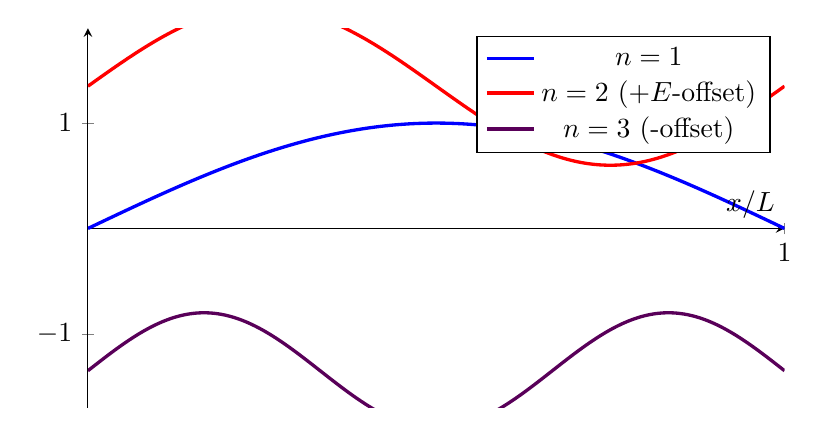
\begin{tikzpicture}
\begin{axis}[width=0.86\linewidth,height=6.4cm,xlabel={$x/L$},ylabel={},
 axis lines=middle,domain=0:1,samples=300,ymin=-1.7,ymax=1.9,xtick={0,1}]
 \addplot[blue,very thick,domain=0:1]{sin(deg(pi*x))};
 \addlegendentry{$n=1$};
 \addplot[red,very thick,domain=0:1]{sin(deg(2*pi*x))*0.75+1.35};
 \addlegendentry{$n=2$ (+$E$-offset)};
 \addplot[violet!70!black,very thick,domain=0:1]{sin(deg(3*pi*x))*0.55-1.35};
 \addlegendentry{$n=3$ (-offset)};
\end{axis}
\end{tikzpicture}
\caption{અનંત કૂવાનાં $\psi_n$; નોડો $n-1$ સંખ્યામાં.}
\end{figure}

\subsection*{આકૃતિ 4.2 : પગથિયું અને અવરોધ — સ્થિતિઊર્જા ચિત્રો}
\begin{figure}[htbp]
\centering
\begin{tikzpicture}[scale=0.95]
 \draw[thick,-Stealth] (-3.5,0) -- (3.5,0);
 % step
 \draw[blue,very thick] (-3.5,0.15) -- (0,0.15) -- (0,1.6) -- (3.5,1.6);
 \node[blue] at (-2,0.45) {$V=0$};
 \node[blue] at (2.2,1.85) {$V=V_0$};
 \draw[dashed,red] (-3.5,0.9) node[left] {$E>V_0$} -- (3.5,0.9);
 \node at (0,-0.4) {(a) પગથિયું};
 % barrier
 \begin{scope}[shift={(0,-3.4)}]
 \draw[thick,-Stealth] (-3.5,0) -- (3.5,0);
 \fill[orange!30] (-0.8,0.15) rectangle (0.8,1.9);
 \draw[orange!70!black,very thick] (-3.5,0.15) -- (-0.8,0.15) -- (-0.8,1.9) -- (0.8,1.9) -- (0.8,0.15) -- (3.5,0.15);
 \node[orange!70!black] at (0,2.15) {$V_0$};
 \draw[<->] (-0.8,-0.25) -- node[below]{$L$} (0.8,-0.25);
 \draw[dashed,red] (-3.5,0.8) node[left] {$E<V_0$} -- (3.5,0.8);
 \node at (0,-0.75) {(b) અવરોધ — ટનલિંગ};
 \end{scope}
\end{tikzpicture}
\caption{પગથિયું અને અવરોધ સ્થિતિઊર્જા સંરચનાઓ.}
\end{figure}

\subsection*{આકૃતિ 4.3 : ટનલિંગ — $T$ vs $L$ (ઘાતાંકીય)}
\begin{figure}[htbp]
\centering
\begin{tikzpicture}
\begin{axis}[width=0.62\linewidth,height=5.6cm,xlabel={$L$ (Å)},ylabel={$T$ (પ્રમાણભૂત)},
 axis lines=box,domain=0:10,samples=120,ymin=0]
 \addplot[blue,very thick]{exp(-1.05*x)};
 \addplot[red,dashed,very thick]{exp(-0.52*x)};
 \legend{ઇલેક્ટ્રોન ($V_0-E=2$ eV), પ્રોટોન (હલકો ઢાળ)}
\end{axis}
\end{tikzpicture}
\caption{$T\propto e^{-2\alpha L}$ — પહોળાઈ/દળ વધે તો ટનલિંગ પ્રચંડ રીતે ઘટે.}
\end{figure}

\subsection*{આકૃતિ 4.4 : STMનું સ્કીમેટિક}
\begin{figure}[htbp]
\centering
\begin{tikzpicture}[scale=1.0]
 \draw[very thick,gray] (0,2.6) -- (0.5,2.0) -- (0.5,1.55) -- (0.42,1.45);
 \node[right] at (0.6,2.4) {ટંગસ્ટન ટિપ};
 \draw[thick,fill=gray!25] (-1.6,-0.4) rectangle (2.4,0);
 \node[below] at (0.4,-0.45) {વાહક નમૂનો};
 \draw[-Stealth,cyan!60!black,dashed,very thick] (0.46,1.4) -- (0.46,0.05);
 \node[cyan!60!black,left] at (0.4,0.7) {$I\propto e^{-2\kappa z}$};
 \draw[<->,red] (0.75,1.4) -- node[right]{$z$} (0.75,0.02);
 \draw[thick] (0.5,2.0) -- (0.5,3.1);
 \draw[thick,-Stealth] (0.5,3.1) -- (0.5,3.5); \node[right] at (0.55,3.3) {પાઇઝો-સ્કેનર};
 \draw[thick] (-2.6,0.6) circle[radius=0.32]; \node[left] at (-2.95,0.6) {$I$ માપન};
 \draw[thick] (-2.28,0.6) -- (0.44,0.9);
 \draw[thick] (2.4,-0.2) -- (3.2,-0.2) -- (3.2,1.2);
 \draw (3.2,1.2) -- (3.2,1.6); \node[right] at (3.28,1.4) {$V_b$};
\end{tikzpicture}
\caption{STM: ટનલ-ધારાની ઘાતાંકીય દૂર-સંવેદનશીલતાથી પરમાણુ-ટોપોગ્રાફી.}
\end{figure}

\subsection*{આકૃતિ 4.5 : હાર્મોનિક દોલક — સ્થિતિઊર્જા અને સ્તરો}
\begin{figure}[htbp]
\centering
\begin{tikzpicture}
\begin{axis}[width=0.66\linewidth,height=6cm,xlabel={$x$},ylabel={$V,E$},
 axis lines=middle,domain=-3.2:3.2,samples=200,ymin=0,ymax=6,
 xtick=\empty,ytick={0.5,1.5,2.5,3.5,4.5}]
 \addplot[blue,very thick]{0.5*x*x};
 \draw[green!50!black,thick] (-2.83,4.0) -- (2.83,4.0);
 \draw[red,thick] (-1.73,1.5) -- (1.73,1.5);
 \draw[orange!80!black,thick] (-1.0,0.5) -- (1.0,0.5);
 \node[orange!80!black,right] at (1.1,0.5) {$E_0=\tfrac12\hbar\omega$};
 \node[red,right] at (1.85,1.5) {$E_1=\tfrac32\hbar\omega$};
 \node[green!50!black,right] at (2.95,4.0) {$E_3$};
\end{axis}
\end{tikzpicture}
\caption{દોલકની પરવલયિક સ્થિતિઊર્જા અને સમાન-અંતર ઊર્જા-સિડી $(n+\tfrac12)\hbar\omega$.}
\end{figure}

\section{સંપૂર્ણ ઉકેલેલા દાખલા}
\begin{dahlo}{દાખલો 4.1 : કૂવાની ભૂમિ-ઊર્જા}
ઇલેક્ટ્રોન $L=1$ Å કૂવામાં બંધનિત છે. $E_1$ અને $E_2$ ગણો.
\tcblower
\textbf{ઉકેલ:} $\dfrac{\pi^{2}\hbar^{2}}{2mL^{2}}=\dfrac{9.87\times(1.055\times10^{-34})^{2}}{2\times9.11\times10^{-31}\times10^{-20}}=6.03\times10^{-18}$ J $=37.6$ eV.
$E_1=37.6$ eV; $E_2=4E_1=150.4$ eV; સંક્રમણ ઊર્જા $112.8$ eV (XUV પ્રદેશ).
\end{dahlo}

\begin{dahlo}{દાખલો 4.2 : 3D બોક્સની ક્ષીણતા}
ઘન બોક્સમાં $E=14E_0$ ઊર્જાની કેટલી અવસ્થાઓ? ($E_0=\pi^2\hbar^2/2mL^2$)
\tcblower
\textbf{ઉકેલ:} $n_x^{2}+n_y^{2}+n_z^{2}=14$ શોધીએ: $1^{2}+2^{2}+3^{2}=14$. ક્રમ-વિનિમય: $(1,2,3)$ નાં $3!=6$ ક્રમ. એટલે $g=6$.
(સરખામણી: $E=6E_0\Rightarrow g=3$; $E=3E_0\Rightarrow(1,1,1)\Rightarrow g=1$.)
\end{dahlo}

\begin{dahlo}{દાખલો 4.3 : પરિમિત કૂવામાં પ્રસરણ અંતર}
ઇલેક્ટ્રોનની ઊર્જા $V_0-E=1$ eV હોય તો પ્રસરણ અંતર $\delta=1/\alpha$ ગણો.
\tcblower
\textbf{ઉકેલ:} $\alpha=\sqrt{2m(V_0-E)}/\hbar$
\[
=\frac{\sqrt{2\times9.11\times10^{-31}\times1.602\times10^{-19}}}{1.055\times10^{-34}}
=\frac{5.40\times10^{-25}}{1.055\times10^{-34}}=5.12\times10^{9}\ \mathrm{m}^{-1}.
\]
$\delta=1/\alpha=1.95\times10^{-10}$ m $\approx2$ Å — પરમાણુ-ક્રમનું પ્રસરણ!
\end{dahlo}

\begin{dahlo}{દાખલો 4.4 : પગથિયું $E>V_0$ માટે $R,T$}
ઇલેક્ટ્રોન $E=5$ eV, $V_0=4$ eV પગથિયા પર પડે. $R$ અને $T$ ગણો.
\tcblower
\textbf{ઉકેલ:} $k\propto\sqrt{E-V}$ ધારવાથી $k_2/k_1=\sqrt{(5-4)/5}=0.447$.
\[
R=\left(\frac{1-0.447}{1+0.447}\right)^{2}=\left(\frac{0.553}{1.447}\right)^{2}=0.146,
\qquad
T=\frac{4(0.447)}{(1.447)^{2}}=0.854 .
\]
શાસ્ત્રીય ભવિષ્યવાણી $R=0$; ક્વોન્ટમ $R\approx15\%$ — ઊર્જા સંરક્ષણ સાથે $R+T=1$. ✓
\end{dahlo}

\begin{dahlo}{દાખલો 4.5 : ટનલિંગ સંભાવના}
ઇલેક્ટ્રોન $E=2$ eV, $V_0=5$ eV, $L=10$ Å અવરોધ પાર કરે તો $T$ ગણો.
\tcblower
\textbf{ઉકેલ:} $V_0-E=3$ eV:
\[
\alpha=\frac{\sqrt{2\times9.11\times10^{-31}\times3\times1.602\times10^{-19}}}{1.055\times10^{-34}}
=8.87\times10^{9}\ \mathrm{m}^{-1};
\qquad 2\alpha L=2(8.87\times10^{9})(10^{-9})=17.74 .
\]
પૂર્વ-ગુણક: $\dfrac{16E(V_0-E)}{V_0^{2}}=\dfrac{16\times2\times3}{25}=3.84$:
\[
T=3.84\times e^{-17.74}=3.84\times1.97\times10^{-8}=7.6\times10^{-8}.
\]
એટલે લગભગ $1.3\times10^{7}$ ઇલેક્ટ્રોનમાંથી એક જ પાર જાય — છતાં STM માં આ જ પ્રક્રિયા nA ધારા આપે!
\end{dahlo}

\begin{dahlo}{દાખલો 4.6 : $\alpha$-ક્ષયની આયુ-સંવેદનશીલતા}
ગામોવ સિદ્ધાંત મુજબ $T\sim e^{-2G}$. $2G$ 30 થી 31 થાય તો આયુ કેટલા ગણી બદલાય?
\tcblower
\textbf{ઉકેલ:} આયુ $t\propto1/T\sim e^{+2G}$: ગુણોત્તર $=e^{31-30}=e\approx2.72$.
એક એકમનો ફેરફાર ≈ ત્રણ-ગણ આયુ-ફેરફાર; $^{238}$U જેવાં ન્યુક્લાઇડમાં $2G\approx90$ ⇒ આયુ $10^{17}$ s (અર્ધ-આયુ $4.5\times10^{9}$ વર્ષ) — નાના $G$-ફેરફારો મહાકલ્પીય તફાવત કરે.
\end{dahlo}

\begin{dahlo}{દાખલો 4.7 : STM ધારા-સંવેદનશીલતા}
ટિપ–સપાટી અંતર $1$ nm થી $1.2$ nm થાય તો ટનલ ધારા કેટલા ગણી બદલાય? ($\kappa\approx10^{10}\ \mathrm{m}^{-1}$)
\tcblower
\textbf{ઉકેલ:} $I\propto e^{-2\kappa z}$:
\[
\frac{I_2}{I_1}=e^{-2\kappa(z_2-z_1)}=e^{-2\times10^{10}\times0.2\times10^{-9}}=e^{-4}=0.018 .
\]
ધારા ≈ 55 ગણી ઘટે — એક હાઇડ્રોજન પરમાણુ જેટલા (0.2 nm) અંતર-ફેરફારથી ધારામાં પ્રચંડ ફેરફાર.
\end{dahlo}

\begin{dahlo}{દાખલો 4.8 : દોલકનું ભૂમિ-તરંગ વિધેય}
$\psi_0=N_0e^{-\xi^{2}/2}$ પ્રમાણિત કરો અને $N_0$ શોધો ($a\equiv\sqrt{\hbar/m\omega}$).
\tcblower
\textbf{ઉકેલ:} $\xi=x/a$, $P=N_0^{2}e^{-x^{2}/a^{2}}$:
\[
1=N_0^{2}\int_{-\infty}^{\infty}e^{-x^{2}/a^{2}}\dd x=N_0^{2}\,a\sqrt{\pi}
\Rightarrow N_0=\frac{1}{(\pi a^{2})^{1/4}}=\frac{1}{\pi^{1/4}\sqrt{a}} .
\]
તપાસ: TISE માં $\psi_0$ રાખતાં $E_0=\hbar\omega/2$ મળે — શૂન્ય-બિંદુ ઊર્જા ફરી પુષ્ટ.
\end{dahlo}

\begin{dahlo}{દાખલો 4.9 : હાઇડ્રોજનનાં અવસ્થા-ગણતરી}
$n=3$ અવસ્થા માટે (a) શક્ય $\ell$ મૂલ્યો, (b) દરેક $\ell$ માટે $m_\ell$, (c) કુલ ક્ષીણતા (સ્પિન વિના) શોધો.
\tcblower
\textbf{ઉકેલ:} (a) $\ell=0,1,2$.
(b) $\ell=0$: $m_\ell=0$ (1 અવસ્થા); $\ell=1$: $m_\ell=-1,0,+1$ (3); $\ell=2$: $m_\ell=-2..+2$ (5).
(c) કુલ $=1+3+5=9=n^{2}$. ✓ સ્પિન સહિત $g=18$.
\end{dahlo}

\begin{dahlo}{દાખલો 4.10 : હાઇડ્રોજન સંક્રમણ તરંગલંબાઈ}
$n=4\to n=2$ સંક્રમણની ઉત્સર્જિત તરંગલંબાઈ ગણો.
\tcblower
\textbf{ઉકેલ:} $E_4=-13.6/16=-0.85$ eV; $E_2=-3.40$ eV; $\Delta E=2.55$ eV.
\[
\lambda=\frac{1240\ \text{eV·nm}}{2.55\ \text{eV}}=486\ \text{nm}.
\]
આ જ પ્રખ્યાત બેલ્મર H$\beta$ નીલમ રેખા છે.
\end{dahlo}

\section{સ્વાધ્યાય}

\subsection{વૈચારિક પ્રશ્નો}
\begin{enumerate}[label=\textbf{Q\arabic*.}]
  \item અનંત કૂવાની ઊર્જા શા માટે અસતત છે જ્યારે મુક્ત કણની સતત?
  \item કૂવાની પહોળાઈ ઘટાડવાથી ઊર્જા-સ્તરો પર શું થાય?
  \item 3D બોક્સમાં ક્ષીણતા 1D કેમ નથી?
  \item પરિમિત કૂવાનાં ઊર્જા-સ્તરો અનંત કૂવા કરતાં નાના કેમ?
  \item $E>V_0$ પગથિયા પર પરાવર્તન શાસ્ત્રીય અંતર્દૃષ્ટિને કેવી રીતે વિરોધાભાસી છે?
  \item ટનલિંગ દર પર દળ અને અવરોધ-પહોળાઈની ઘાતાંકીય અસર સમજાવો.
  \item STM માં ધારા કેમ 'પરમાણુ-ઊંચાઈ' માપે છે?
  \item શૂન્ય-બિંદુ ઊર્જા દોલકમાં અનિશ્ચિતતા સિદ્ધાંતથી કેમ અનિવાર્ય છે?
  \item હાઇડ્રોજનમાં $n$ જ ઊર્જા નક્કી કરે પણ $\ell,m_\ell$ કેમ જરૂરી?
  \item કૂલુંબ-અવરોધનું ટનલિંગ સૂર્યનાં ફ્યુઝન માટે કેમ અનિવાર્ય છે?
\end{enumerate}

\subsection{અણઉકેલેલા દાખલા}
\begin{enumerate}[label=\textbf{P\arabic*.}]
  \item ઇલેક્ટ્રોન, $L=2$ Å કૂવાની $E_1$ ગણો. \hfill [\textbf{જવાબ:} $9.4$ eV]
  \item P1 માં $n=3\to1$ સંક્રમણ ફોટોનનું $\lambda$ ગણો. \hfill [\textbf{જવાબ:} $\approx11$ nm]
  \item ઘન બોક્સમાં $E=12E_0$ ની ક્ષીણતા ગણો. \hfill [\textbf{જવાબ:} $g=1$ ($(2,2,2)$)]
  \item $V_0-E=2$ eV ઇલેક્ટ્રોન માટે $\delta$ ગણો. \hfill [\textbf{જવાબ:} $\approx1.4$ Å]
  \item $E=6$ eV, $V_0=4$ eV પગથિયાનું $R$ ગણો. \hfill [\textbf{જવાબ:} $\approx0.036$]
  \item $E=3$ eV, $V_0=6$ eV, $L=5$ Å અવરોધનું $T$ ગણો. \hfill [\textbf{જવાબ:} $\sim10^{-5}$ ક્રમ]
  \item STM અંતર $0.5\to0.6$ nm: ધારા-ગુણોત્તર ($\kappa=10^{10}$). \hfill [\textbf{જવાબ:} $\approx0.135$]
  \item દોલક $n=2$ નાં નોડ-સંખ્યા અને ઊર્જા લખો. \hfill [\textbf{જવાબ:} 2 નોડ; $E_2=\tfrac52\hbar\omega$]
  \item હાઇડ્રોજન $n=2$: ક્ષીણતા (સ્પિન સહિત) ગણો. \hfill [\textbf{જવાબ:} $8$]
  \item હાઇડ્રોજન $n=3\to2$ સંક્રમણ $\lambda$ ગણો. \hfill [\textbf{જવાબ:} $656$ nm (H$\alpha$)]
\end{enumerate}

\section{50 ઉચ્ચ સ્તરીય MCQs}

\begin{enumerate}[label=\textbf{\arabic*.}]
  \item અનંત કૂવાની ઊર્જા $E_n\propto$ ? (A) $n$ (B) $n^{2}$ (C) $n^{3}$ (D) $1/n$
  \item કૂવાની ભૂમિ-અવસ્થા ઊર્જા: (A) 0 (B) $\pi^{2}\hbar^{2}/2mL^{2}$ (C) $\infty$ (D) $\hbar^{2}/2mL^{2}$
  \item $\psi_n$ નાં નોડ (કૂવા અંદર): (A) $n$ (B) $n-1$ (C) $n+1$ (D) $2n$
  \item કૂવાની પહોળાઈ અડધી થાય તો $E_1$: (A) અડધું (B) બમણું (C) ચાર-ગણું (D) અપરિવર્તિત
  \item પ્રમાણિત $\psi_n$ નો $A=$ ? (A) $1/\sqrt L$ (B) $\sqrt{2/L}$ (C) $2/L$ (D) $\sqrt{L/2}$
  \item 3D ઘન બોક્સ $E=6E_0$ ની ક્ષીણતા: (A) 1 (B) 3 (C) 6 (D) 9
  \item 3D ઘન બોક્સ $E=3E_0$ ની ક્ષીણતા: (A) 1 (B) 3 (C) 6 (D) 8
  \item પરિમિત કૂવાનાં ઊર્જા-સ્તરો મળે છે: (A) બીજગણિતથી (B) અતિચલાંકીય સમીકરણોના સંખ્યાત્મક ઉકેલથી (C) અનંત-કૂવા જેવા જ (D) શૂન્ય
  \item પ્રસરણ અંતર $\delta=$ ? (A) $\hbar/\sqrt{2m(V_0-E)}$ (B) $\sqrt{2mV_0}/\hbar$ (C) $\alpha$ (D) $2\alpha L$
  \item કૂવાની બહાર $|\psi|$ નું સ્વરૂપ: (A) દોલાતું (B) ઘાતાંકીય ક્ષય (C) રેખીય (D) શૂન્ય
  \item $E>V_0$ પગથિયા પર ક્વોન્ટમ પરિણામ: (A) $R=0$ (B) $R>0$ (C) $T=0$ (D) $R=1$
  \item પગથિયું $E\to V_0$ (ઉપરથી) મર્યાદામાં $R\to$ ? (A) 0 (B) 1 (C) 0.5 (D) $\infty$
  \item પગથિયું $E\gg V_0$ માં $R\approx$ ? (A) 1 (B) 0.5 (C) $\approx0$ (D) $V_0/E$
  \item $E<V_0$ અનંત પગથિયા માટે $T=$ ? (A) $e^{-2\alpha L}$ (B) 0 (C) 1 (D) $V_0/E$
  \item અવરોધ ટનલિંગ $T\approx$ ? (A) $e^{-2\alpha L}$ (B) $e^{+2\alpha L}$ (C) $\alpha L$ (D) $1/\alpha L$
  \item $\alpha=$ ? (A) $\sqrt{2m(E-V_0)}/\hbar$ (B) $\sqrt{2m(V_0-E)}/\hbar$ (C) $2mV_0/\hbar$ (D) $\hbar/\sqrt{2mV_0}$
  \item અવરોધ-પહોળાઈ બમણી થાય તો $T$ લગભગ: (A) બમણું (B) અડધું (C) $T$ નું વર્ગ ઘટે ($e^{-4\alpha L}$) (D) અપરિવર્તિત
  \item ગામોવ સિદ્ધાંત સમજાવે છે: (A) ફોટોવિદ્યુત અસર (B) $\alpha$-ક્ષયની આયુ (C) લેસર (D) સુપરકંડક્ટન્સ
  \item $\alpha$-ક્ષયમાં કણ કેવી રીતે છટકે? (A) કૂલુંબ-અવરોધનું ટનલિંગ (B) ગુરુત્વ (C) ફોટોન શોષણ (D) માગ્નેટિક ક્ષેત્ર
  \item Geiger-Nuttall નિયમ સંકળાયેલ: (A) $\alpha$-ક્ષય આયુ–ઊર્જા (B) β-વર્ણપટ (C) γ-શોષણ (D) ફ્યુઝન-દર
  \item STM ના શોધક: (A) બેલ-બિનિંગ (B) બિનિંગ-રોહરર (C) ડેવિસન-જર્મર (D) થોમસન
  \item STM ધારા સ્વરૂપ: (A) $e^{-2\kappa z}$ (B) $z^{2}$ (C) $1/z$ (D) $e^{+2\kappa z}$
  \item ટનલ ડાયોડની વિશિષ્ટ વિશેષતા: (A) ધન પ્રતિરોધ (B) નેગેટિવ ડિફરેન્શિયલ રેઝિસ્ટન્સ (C) અનંત પ્રતિરોધ (D) શૂન્ય ધારા
  \item ફ્લેશ મેમરીમાં ચાર્જ-ઇન્જેક્શન પ્રક્રિયા: (A) થર્મિયોનિક (B) ફોવલર-નોર્ધામ ટનલિંગ (C) ફોટોવિદ્યુત (D) કૉમ્પ્ટન
  \item દોલકની ઊર્જા સિડી: (A) સમાન-અંતર $\hbar\omega$ (B) $n^{2}$ પ્રમાણે (C) સતત (D) $1/n^{2}$
  \item દોલકની શૂન્ય-બિંદુ ઊર્જા: (A) 0 (B) $\hbar\omega$ (C) $\hbar\omega/2$ (D) $3\hbar\omega/2$
  \item દોલક તરંગ-વિધેયમાં બહુપદી: (A) લાગ્યુર (B) હર્માઇટ (C) લેજાન્ડર (D) ચેબિશેવ
  \item $H_2(\xi)=$ ? (A) $2\xi$ (B) $4\xi^{2}-2$ (C) $1$ (D) $8\xi^{3}-12\xi$
  \item દોલકની ભૂમિ-અવસ્થાનાં નોડ: (A) 0 (B) 1 (C) 2 (D) $\infty$
  \item હાઇડ્રોજન ઊર્જા $E_n$ આધારિત છે: (A) ફક્ત $n$ પર (B) ફક્ત $\ell$ પર (C) $m_\ell$ પર (D) ત્રણેય પર
  \item હાઇડ્રોજન માટે શક્ય $\ell$: (A) $\ell<n$ (B) $\ell\le n$ (C) $\ell>n$ (D) $\ell=n^{2}$
  \item હાઇડ્રોજન માટે શક્ય $m_\ell$: (A) $|m_\ell|\le\ell$ (B) $|m_\ell|\le n$ (C) કોઈપણ પૂર્ણાંક (D) $\pm1$
  \item સ્પિન ક્વોન્ટમ સંખ્યા $m_s=$ ? (A) $\pm\tfrac12$ (B) $0,1$ (C) $\pm1$ (D) $n$
  \item હાઇડ્રોજન $n$-અવસ્થાની ક્ષીણતા (સ્પિન વિના): (A) $n$ (B) $2n^{2}$ (C) $n^{2}$ (D) $n^{3}$
  \item હાઇડ્રોજન ભૂમિ-અવસ્થાની $\ell$: (A) 0 (B) 1 (C) $n-1$ (D) કોઈ નહીં
  \item બેલ્મર H$\alpha$ ($656$ nm) સંક્રમણ: (A) $3\to2$ (B) $4\to2$ (C) $2\to1$ (D) $5\to2$
  \item લાયમન શ્રેણી પ્રદેશ: (A) IR (B) દૃશ્ય (C) UV (D) X-ray
  \item કૂવાની ઊર્જા-સ્પેસિંગ મોટા $n$ પર: (A) વધે (B) ઘટે અને લગભગ સતત જેવી (C) અચલાંક (D) અનંત
  \item અનંત કૂવાની સીમા પર $\psi$: (A) મહત્તમ (B) 0 (C) અનંત (D) $1/L$
  \item પગથિયા પર $\psi$ અને $\psi'$: (A) અસતત (B) સતત (C) એક જ સતત (D) શૂન્ય
  \item ટનલિંગ શા માટે શાસ્ત્રીયમાં અશક્ય? (A) $E<V_0$ પ્રદેશમાં $p$ કાલ્પનિક (B) ઊર્જા અભાવ (C) દળ વધુ (D) ઝડપ ઓછી
  \item ટનલિંગની સંભાવના સૌથી વધુ જ્યારે: (A) દળ ઓછો, અવરોધ પાતળો (B) દળ મોટો (C) અવરોધ પહોળો (D) ઊર્જા નાની
  \item ક્વોન્ટમ કૂવા-લેસરનું સિદ્ધાંત-આધાર: (A) અનંત કૂવાની અસતત સ્તરો (સ્તર-સંરચના) (B) ટનલિંગ (C) સ્પિન (D) ક્ષીણતા
  \item હાઇડ્રોજન રેડિયલ સંભાવના મહત્તમ (ભૂમિ-અવસ્થા) ત્રિજ્યા: (A) $a_0$ (B) $2a_0$ (C) $a_0/2$ (D) $4a_0$
  \item દોલકમાં શાસ્ત્રીય-ટર્નિંગ બિંદુ એટલે: (A) $V=E$ (B) $V=0$ (C) $\psi=0$ (D) નોડ
  \item WKB ટનલિંગ અંદાજ $T\sim$: (A) $e^{-2\int\alpha dx}$ (B) $\int\alpha dx$ (C) $e^{+\int\alpha dx}$ (D) $\alpha^{2}$
  \item અનંત કૂવામાં $\langle x\rangle$ ($0<x<L$): (A) $0$ (B) $L/2$ (C) $L$ (D) $nL/\pi$
  \item પરિમિત કૂવો જેટલો ઊંડો તેનાં સ્તરો: (A) અનંત કૂવા જેવા (B) અનંત કૂવા કરતાં ઓછા અને નાના ઊર્જા (C) વધુ (D) સતત
  \item હાઇડ્રોજન TISE ગોળીય નિર્દેશાંક કેમ? (A) સરળ ગણિત (B) સ્થિતિઊર્જા કેન્દ્રીય-સમિતિય (C) ક્વોન્ટમ નિયમ (D) સ્પિન જરૂરી
  \item $n=2$ હાઇડ્રોજન અવસ્થાની ઊર્જા: (A) $-13.6$ eV (B) $-3.4$ eV (C) $-1.51$ eV (D) $-0.85$ eV
\end{enumerate}

\subsection*{જવાબ ચાવી અને પગલાંવાર સમજૂતી}
\begin{javabchavi}{MCQ જવાબ ચાવી (એકમ 4)}
1-B | 2-B | 3-B | 4-C | 5-B | 6-B | 7-A | 8-B | 9-A | 10-B |
11-B | 12-B | 13-C | 14-B | 15-A | 16-B | 17-C | 18-B | 19-A | 20-A |
21-B | 22-A | 23-B | 24-B | 25-A | 26-C | 27-B | 28-B | 29-A | 30-A |
31-A | 32-A | 33-A | 34-C | 35-A | 36-A | 37-C | 38-B | 39-B | 40-B |
41-A | 42-A | 43-A | 44-A | 45-A | 46-B | 47-A | 48-B | 49-B | 50-B
\end{javabchavi}

\begin{javabchavi}{MCQ પગલાંવાર સમજૂતી (મુખ્ય ગણતરી-આધારિત પ્રશ્નો)}
\begin{description}[style=nextline,itemsep=0pt]
  \item[4.] $E_1\propto1/L^{2}$; $L\to L/2$ ⇒ $E_1\to4E_1$.
  \item[6./7.] $n_x^{2}+n_y^{2}+n_z^{2}$: $6=(1,1,\sqrt4)=(1,1,2)$ ત્રણ ક્રમ ⇒ $g=3$; $3=(1,1,1)$ ⇒ $g=1$.
  \item[9.] $\delta=1/\alpha=\hbar/\sqrt{2m(V_0-E)}$ — $|\psi|$ નું $e^{-1}$ ભાગનું અંતર.
  \item[11.] $E>V_0$: $R=\big((k_1-k_2)/(k_1+k_2)\big)^{2}>0$ જ્યારે $k_2\neq k_1$ — ક્વોન્ટમ પરાવર્તન.
  \item[12.] $E\to V_0$: $k_2\to0$ ⇒ $R\to1$ — સંપૂર્ણ પરાવર્તન મર્યાદા.
  \item[17.] $L\to2L$: $e^{-2\alpha(2L)}=(e^{-2\alpha L})^{2}$ — વર્ગ ઘટાડો.
  \item[34.] સ્પિન વિના ક્ષીણતા $=\sum_{\ell=0}^{n-1}(2\ell+1)=n^{2}$.
  \item[36.] બેલ્મર H$\beta$: $E_4-E_2=-0.85-(-3.40)=2.55$ eV ⇒ $486$ nm; H$\alpha$ છે $3\to2$.
  \item[44.] ભૂમિ-અવસ્થાની રેડિયલ સંભાવના $P(r)=4r^{2}|\psi_{100}|^{2}/a_0^{3}$ નું મહત્તમ $r=a_0$ પર.
\end{description}
શેષ પ્રશ્નો સૂત્ર-વ્યાખ્યા આધારિત; \S4.2--\S4.3 સાથે સરખાવો.
\end{javabchavi}
